%!TEX root = ./Structure_rapport_final.tex

\subsection{Factorial Analysis of Mixed Data}

The first 5 axis FAMD components explained 78.9\% of the total variation (Table \ref{table:cont_abs}). The first axis (30.6\% of explained variance) is strongly correlated with food acquisition with traits such as \emph{body depth} (a = 12.8), \emph{oral gape axis} (a=11.9), \emph{gill raker type} (a = 11.9), \emph{lower jaw length} (a=10.4) and oral gape surface (a=9.91) (Table \ref{table:cont_abs}). Along this axis, all traits have increasing values toward the right (see \ref{fig:corr_circ_12} for details). As can be seen on Figure \ref{fig:famd12}, this axis clearly separates 3 groups of fishes. At the left, fishes have a low transversal shape (meaning that both \textsc{bd} and \textsc{bw} have similar values, consistent with an elongated body), short lower jaw and small oral gape surface, such as \textit{A. risso}, \textit{S. boa} and \textit{S. beanii}. On the right of this axis, fishes display high body depth values suggesting a laterally compressed form, such as \textit{A. olfersii}. 
The second axis (17.7\% of explained variance) is correlated with food prospection behaviour, through locomotion with \emph{pectoral fin insertion} (a = 15.0), \emph{pectoral fin position} (a = 12.7), which are anti-correlated (see Figure \ref{fig:corr_circ_12}) and diet through \emph{anus position} (a = 10.52) and \emph{oral gape shape} (a = 8.67) (Table \ref{table:cont_abs}). This axis separates the 3 species on the left, \textit{A. risso} diplay higher values of pectoral fin insertion, meaning that the fin is inserted further on the body than \textit{S. boa}, while the fin position on the body depth is lower. Because \textit{S. beanii} does not have pectoral fin, same analysis has been run without traits refering to pectoral or pelvic fins to look if discrimination between species were highly dependant if these traits. Same results than Figure \ref{fig:famd12} were obtained, with \textit{S. boa} and \textit{S. beanii} slightly overlapping. 
The third axis (explaining 13.1\% of total variance) mainly carries traits linked to the habitat and predatory behavior, with strong influence of \emph{oral gape axis} (a = 23.3), \emph{gill raker type} (a = 23.3), \emph{presence of photophores} (a = 11.2) and \emph{caudal throttle width} (a = 10.1) (Table \ref{table:cont_abs}). On the left of this axis (see Figure \ref{fig:famd34}), species are characterized by wide caudal throttle, supra-terminal oral gape axis and `C' gill rakers type (see \ref{fig:oga}), whereas species on the right have a superior oral gape axis and `A' type of gill rakers (see Figure \ref{fig:corr_circ_34}).
+ INTERPRETATION DE L'AXE 4 : operculum volume, anus position, dorsal fin and pyloric caeca --> peut-être en lien avec un comportement de prédateur ou de digestion de proies difficiles ?  

% Table of contributions of variables for 5 first axis
\begin{table}[ht]
\centering
\label{table:cont_abs}
\caption{Correlation bewteen 5 first PC's component and functional traits. In bold, correlations higher than threshold (4.8)}
\begin{adjustbox}{max width=1.1\textwidth,center}
\begin{tabular}{rrrrrr}
  \hline
 & PC1 & PC2 & PC3 & PC4 & PC5 \\ 
  \hline
Eye size & 3.60 & \textbf{8.20} & 2.12 & \textbf{5.14} & 0.80 \\ 
  Orbital length & \textbf{6.03} & \textbf{5.95} & 2.38 & 0.17 & 0.42 \\ 
  Oral gape surface & \textbf{9.91} & 0.32 & 1.16 & 0.60 & 1.56 \\ 
  Oral gape shape & 0.66 & \textbf{8.67} & 1.72 & 3.05 & 3.59 \\ 
  Oral gape position & 0.85 & 1.22 & 0.41 & 4.02 & 0.02 \\ 
  Lower jaw length & \textbf{10.44} & 0.76 & 1.20 & 0.00 & \textbf{5.17} \\ 
  Gill outflow & \textbf{5.82} & 0.01 & 0.00 & 2.21 & \textbf{15.16} \\ 
  Operculum volume & 1.98 & 1.74 & 0.61 & \textbf{18.40} & 4.80 \\ 
  Head length & \textbf{5.00} & \textbf{7.12} & 3.72 & 3.81 & 4.15 \\ 
  Anus position & 0.03 & \textbf{10.52} & 1.81 & \textbf{20.99} & 0.19 \\ 
  Body depth & \textbf{12.80} & 0.25 & 0.35 & 0.06 & 0.10 \\ 
  Pectoral fin position & 0.83 & \textbf{12.72} & 0.00 & \textbf{11.69} & 4.20 \\ 
  Pectoral fin insertion & 1.84 & \textbf{14.96} & \textbf{5.84} & 0.03 & 0.58 \\ 
  Transversal shape & \textbf{8.68} & 0.10 & \textbf{6.30} & 0.48 & 0.00 \\ 
  Caudal throttle width & 1.66 & 3.20 & \textbf{10.09} & 0.18 & \textbf{6.07} \\ 
  Dorsal fin insertion & 3.03 & 4.37 & 0.32 & \textbf{18.04} & \textbf{6.03} \\ 
  Eye position & 0.96 & 3.42 & 3.82 & 0.19 & 3.56 \\ 
  Oral gape axis & \textbf{11.88} & 4.72 & \textbf{23.29} & 0.44 & \textbf{4.86} \\
  Gill raker type & \textbf{11.88} & 4.72 & \textbf{23.29} & 0.44 & \textbf{4.86} \\ 
  Pyloric caeca & 0.34 & 1.27 & 0.42 & \textbf{5.13} & \textbf{26.98} \\ 
  Presence of photophores & 1.82 & \textbf{5.74} & \textbf{11.17} & \textbf{4.92} & \textbf{6.90} \\ 
   \hline
\end{tabular}
\end{adjustbox}
\end{table}

% Or relative values ?
% \begin{table}[ht]
% \centering
% \label{table:cont_abs}
% \caption{Correlation bewteen 5th first PC component and functional traits. In bold, correlations higher than threshold (?????????}
% \begin{adjustbox}{max width=1.1\textwidth,center}
% \begin{tabular}{rrrrrr}
%   \hline
%  & PC1 & PC2 & PC3 & PC4 & PC5 \\ 
%   \hline
% Eye\_size & 0.06 & 0.11 & 0.00 & 0.01 & 0.00 \\ 
%   Orbital\_length & 0.18 & 0.06 & 0.00 & 0.00 & 0.00 \\ 
%   Oral\_gape\_surface & 0.49 & 0.00 & 0.00 & 0.00 & 0.00 \\ 
%   Oral\_gape\_shape & 0.00 & 0.12 & 0.00 & 0.00 & 0.00 \\ 
%   Oral\_gape\_position & 0.00 & 0.00 & 0.00 & 0.01 & 0.00 \\ 
%   Lower\_jaw\_length & 0.54 & 0.00 & 0.00 & 0.00 & 0.01 \\ 
%   Gill\_outflow & 0.17 & 0.00 & 0.00 & 0.00 & 0.08 \\ 
%   Operculum\_volume & 0.02 & 0.00 & 0.00 & 0.15 & 0.01 \\ 
%   Head\_length & 0.12 & 0.08 & 0.01 & 0.01 & 0.01 \\ 
%   Anus\_position & 0.00 & 0.18 & 0.00 & 0.20 & 0.00 \\ 
%   Body\_depth & 0.  & 0.00 & 0.00 & 0.00 & 0.00 \\ 
%   Pectoral\_fin\_position & 0.00 & 0.27 & 0.00 & 0.06 & 0.01 \\ 
%   Pectoral\_fin\_insertion & 0.02 & 0.37 & 0.03 & 0.00 & 0.00 \\ 
%   Transversal\_shape & 0.37 & 0.00 & 0.04 & 0.00 & 0.00 \\ 
%   Caudal\_throttle\_width & 0.01 & 0.02 & 0.09 & 0.00 & 0.01 \\ 
%   Dorsal\_fin\_insertion & 0.04 & 0.03 & 0.00 & 0.15 & 0.01 \\ 
%   Eye\_position & 0.00 & 0.02 & 0.01 & 0.00 & 0.00 \\ 
%   Oral\_gape\_axis & 0.35 & 0.02 & 0.25 & 0.00 & 0.00 \\ 
%   Gill\_raker\_type & 0.35 & 0.02 & 0.25 & 0.00 & 0.00 \\ 
%   Pyloric\_caeca & 0.00 & 0.00 & 0.00 & 0.01 & 0.26 \\ 
%   Presence\_photophores & 0.02 & 0.06 & 0.11 & 0.01 & 0.02 \\ 
%    \hline
% \end{tabular}
% \end{adjustbox}
% \end{table}

% Plot of FAMD axis 1 and 2
\begin{figure} [!htbp]
	\begin{center}
		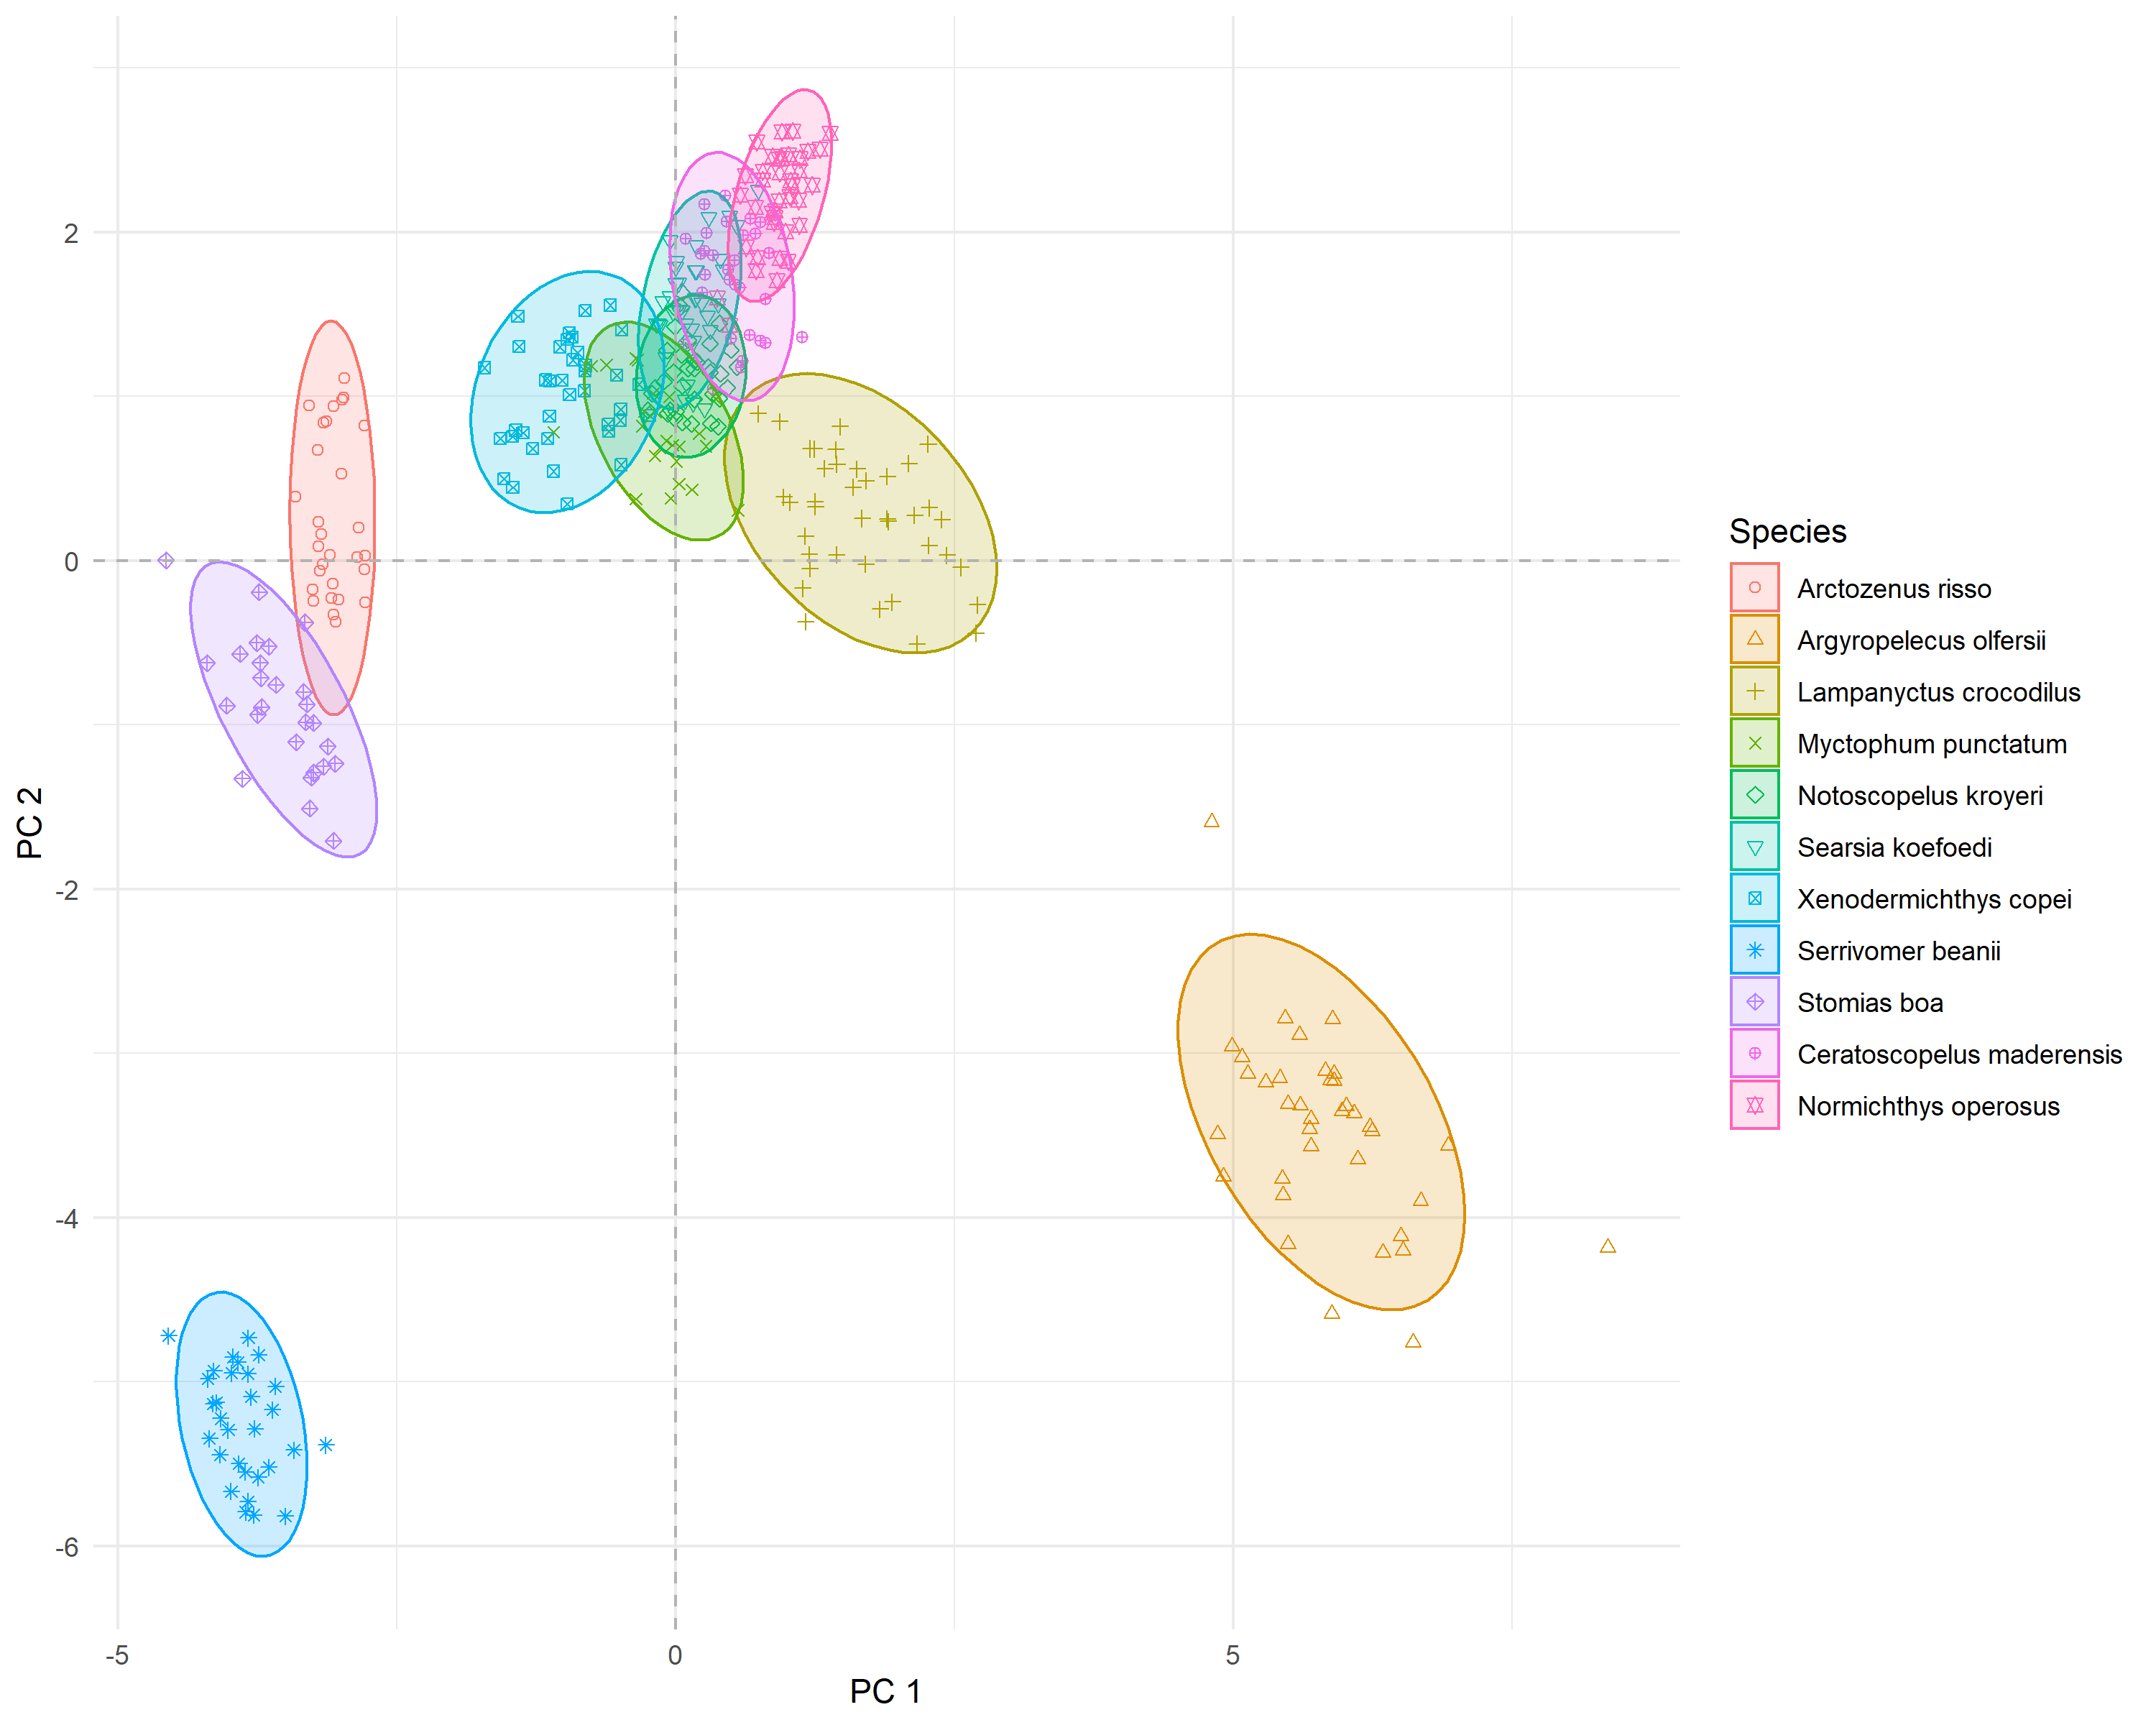
\includegraphics[width=\textwidth]{FAMD_1_2.png}
	\end{center}
	\caption{FAMD results for PC 1 and 2.}
	\label{fig:famd12}
\end{figure}

% Plot of FAMD axis 3 and 4
\begin{figure} [!htbp]
	\begin{center}
		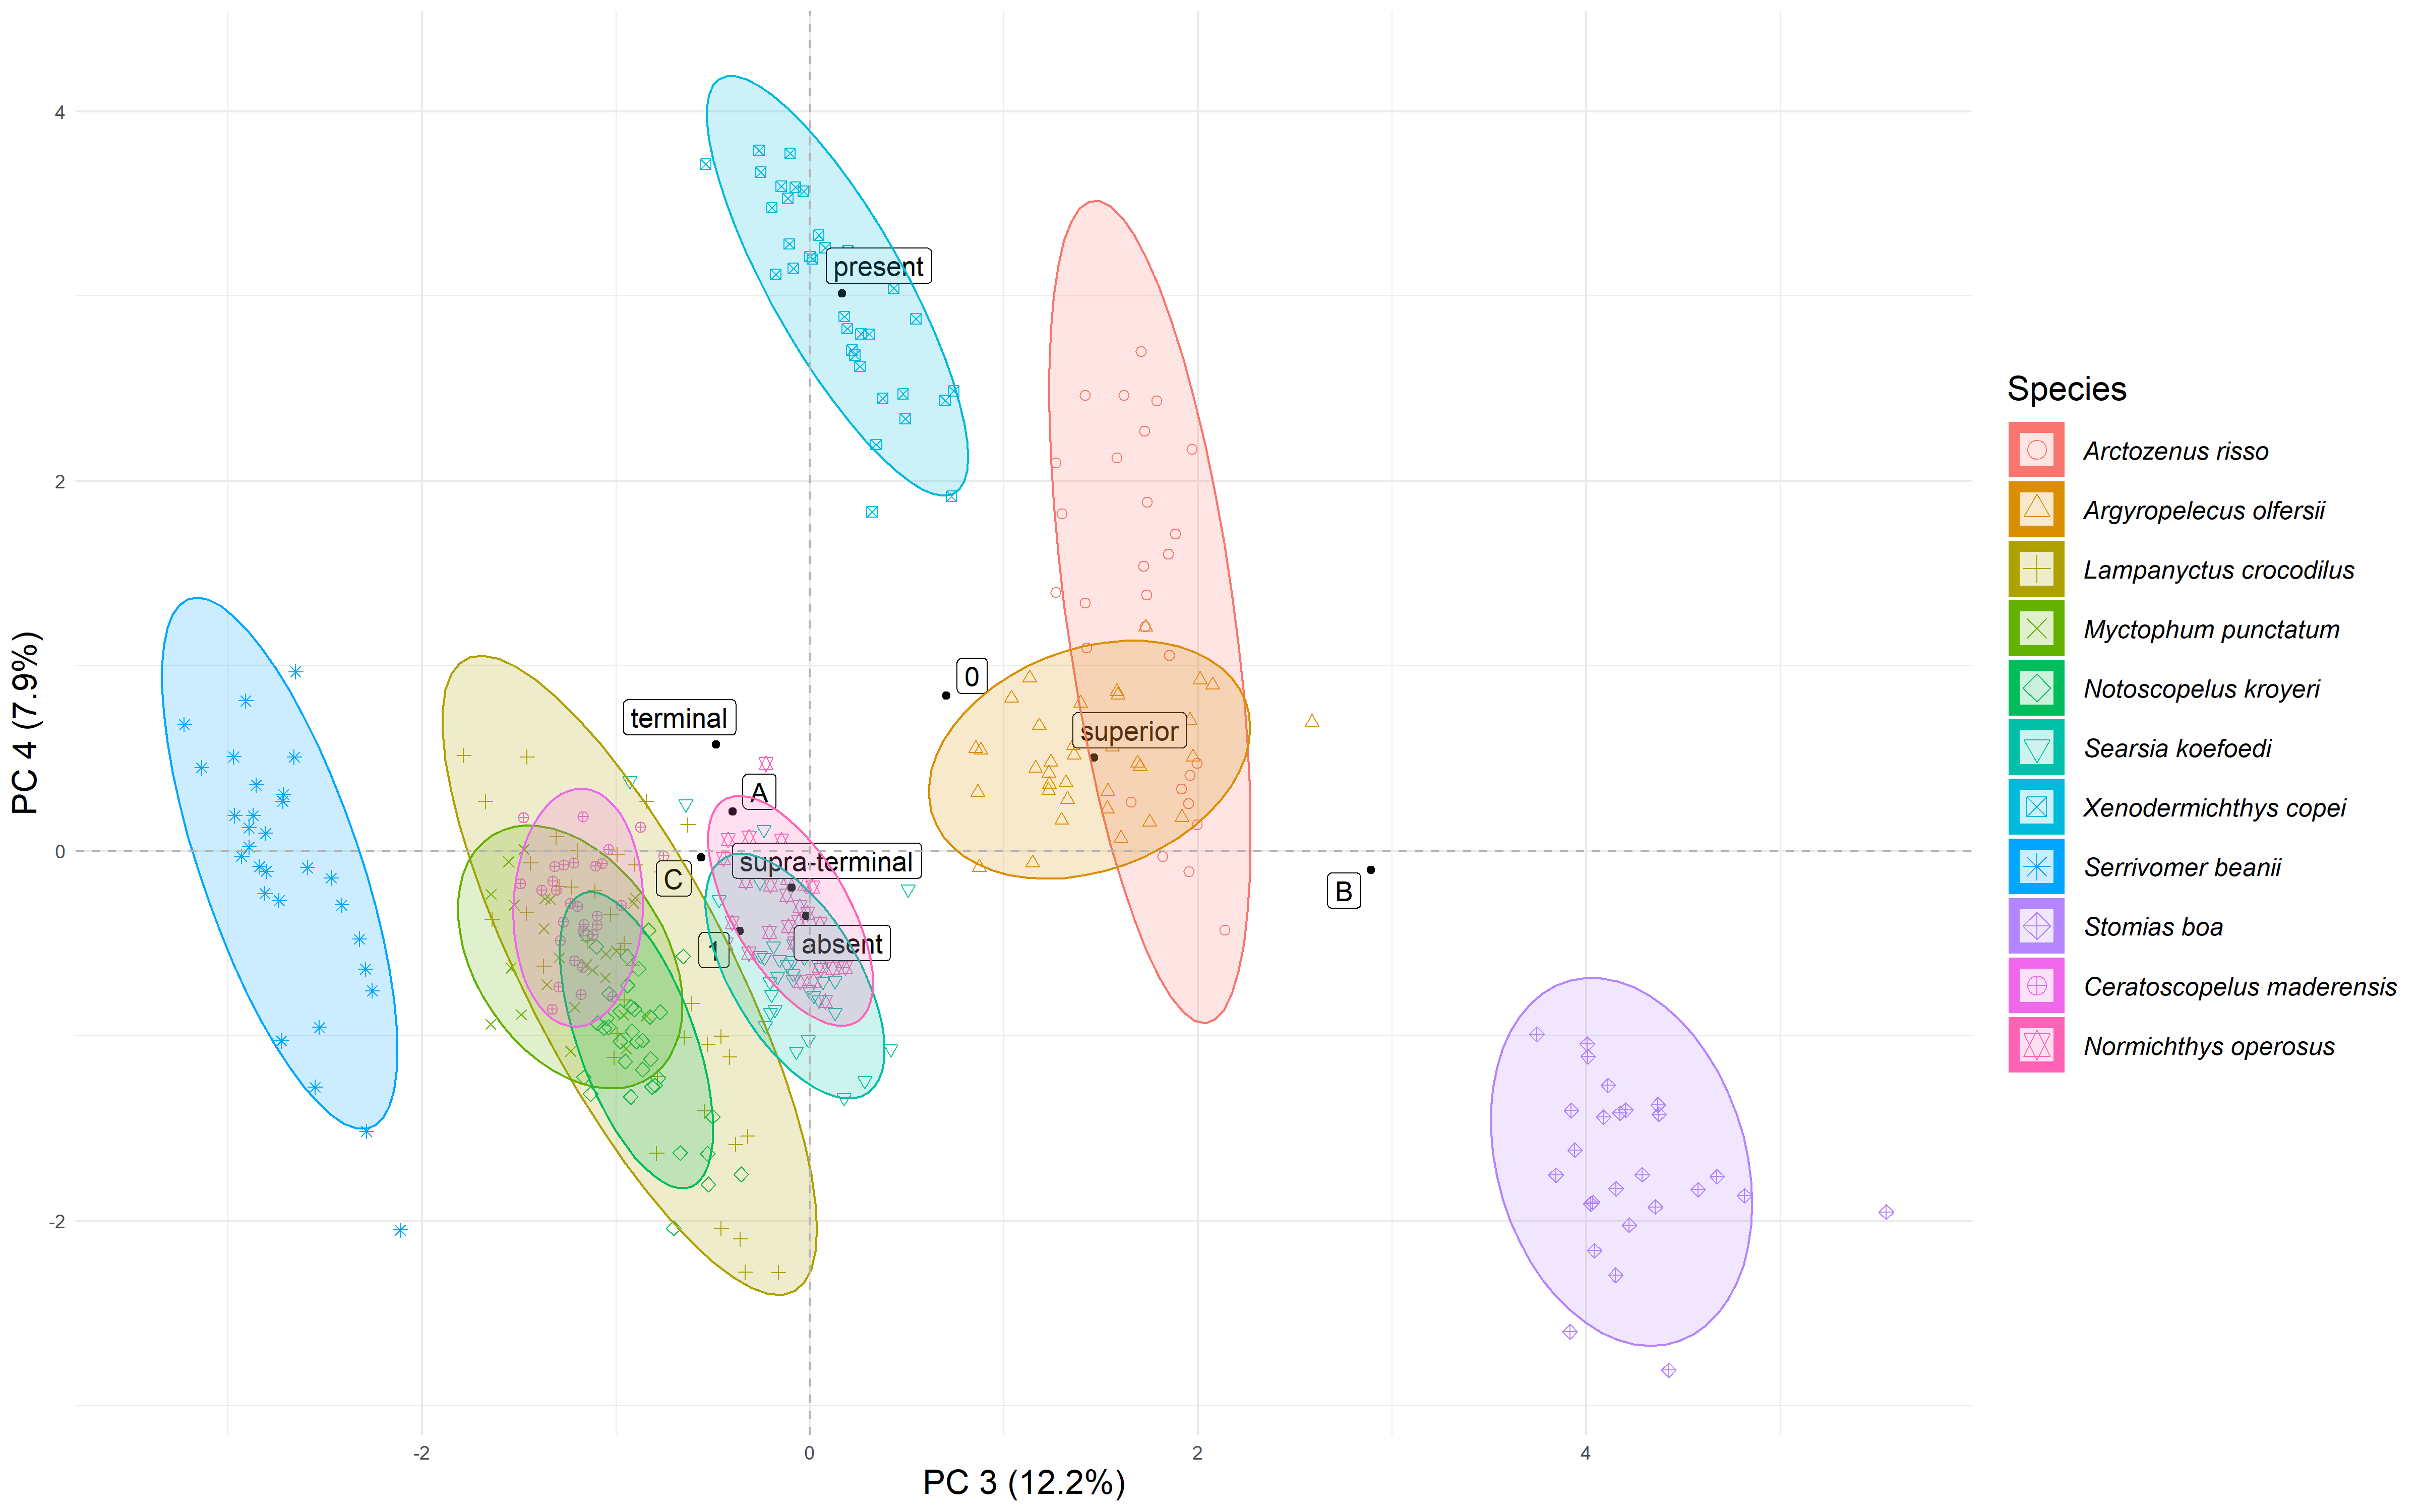
\includegraphics[width=\textwidth]{FAMD_3_4.png}
	\end{center}
	\caption{FAMD results for PC 3 and 4.}
	\label{fig:famd34}
\end{figure}


\subsection{Functional niche area and overlap}

As can be seen on both \ref{fig:famd12} and \ref{fig:famd34}, 6 species present overlapping on the 4 first most discriminant axis, meaning that they are likely to be very much alike. 

% Niche standardardised areas
\begin{table}[ht]
\centering
\label{table:sp_area}
\caption{Standardized area of functional niches.}
\begin{adjustbox}{max width=1.1\textwidth,center}
\begin{tabular}{lr}
  \hline
Species & Area \\ 
  \hline
Argyropelecus olfersii & 5.30 \\ 
  Lampanyctus crocodilus & 3.20 \\ 
  Stomias boa & 2.33 \\ 
  Xenodermichthys copei & 2.14 \\ 
  Arctozenus risso & 2.03 \\ 
  Myctophum punctatum & 1.83 \\ 
  Ceratoscopelus maderensis & 1.80 \\ 
  Serrivomer beanii & 1.73 \\ 
  Searsia koefoedi & 1.10 \\ 
  Normichthys operosus & 1.02 \\ 
  Notoscopelus kroyeri & 1.00 \\ 
   \hline
\end{tabular}
\end{adjustbox}
\end{table}


% Niche overlap 
PROBLEME CHIFFRE SIGNIF.

\begin{table}[ht]
\centering
\label{table:ell_ovlp}
\caption{Species niche overlap}
\begin{adjustbox}{max width=1.1\textwidth,center}
\begin{tabular}{llrrr}
  \hline
Species1 & Species2 & Overlap of Species 2 over Species 1 (\%) & Overlap of Species 1 over Species 2 (\%) & Total overlap (\%)\\ 
  \hline
Notoscopelus kroyeri & Searsia koefoedi & 62.20 & 56.49 & 29.60 \\ 
  Searsia koefoedi & Ceratoscopelus maderensis & 70.63 & 43.30 & 26.84 \\ 
  Myctophum punctatum & Notoscopelus kroyeri & 41.31 & 75.60 & 26.71 \\ 
  Ceratoscopelus maderensis & Normichthys operosus & 29.57 & 51.99 & 18.85 \\ 
  Notoscopelus kroyeri & Ceratoscopelus maderensis & 43.63 & 24.29 & 15.60 \\ 
  Myctophum punctatum & Searsia koefoedi & 22.35 & 37.14 & 13.95 \\ 
  Searsia koefoedi & Normichthys operosus & 15.75 & 16.98 & 8.17 \\ 
  Xenodermichthys copei & Ceratoscopelus maderensis & 13.84 & 16.48 & 7.52 \\ 
  Myctophum punctatum & Ceratoscopelus maderensis & 12.30 & 12.53 & 6.21 \\ 
  Lampanyctus crocodilus & Myctophum punctatum & 8.04 & 14.06 & 5.11 \\ 
  Searsia koefoedi & Xenodermichthys copei & 8.56 & 4.41 & 2.91 \\ 
  Lampanyctus crocodilus & Ceratoscopelus maderensis & 4.51 & 8.04 & 2.89 \\ 
  Lampanyctus crocodilus & Notoscopelus kroyeri & 2.94 & 9.41 & 2.24 \\ 
  Notoscopelus kroyeri & Normichthys operosus & 0.62 & 0.61 & 0.31 \\ 
   \hline
\end{tabular}
\end{adjustbox}
\end{table}


\subsection{Kernel density estimation}
% Plot of density kernel
The estimation of kernel density overlap for functional traits of overlapping species concludes that these species are all overlaping for 11 traits (see figure \ref{fig:dpo}). The overlap is maximum for the position of the oral gape (trait n°5) with an overlap value of 0.338. This means that, along this functional trait, these 6 species share nearly 34\% of their density. Species also share nearly 25\% and 29\% of their density when looking at body depth (trait n°11) and eye position (trait n°17, respectively. Finally, lower jaw length (trait n°6) and pectoral fin position (trait n°12) values also seem to be common to those species, with 16\% and 19\% of density shared, respectively. To a lesser extent, species share 12\% of the eye size values (trait n°2).

\begin{figure} [!htbp]
	\begin{center}
		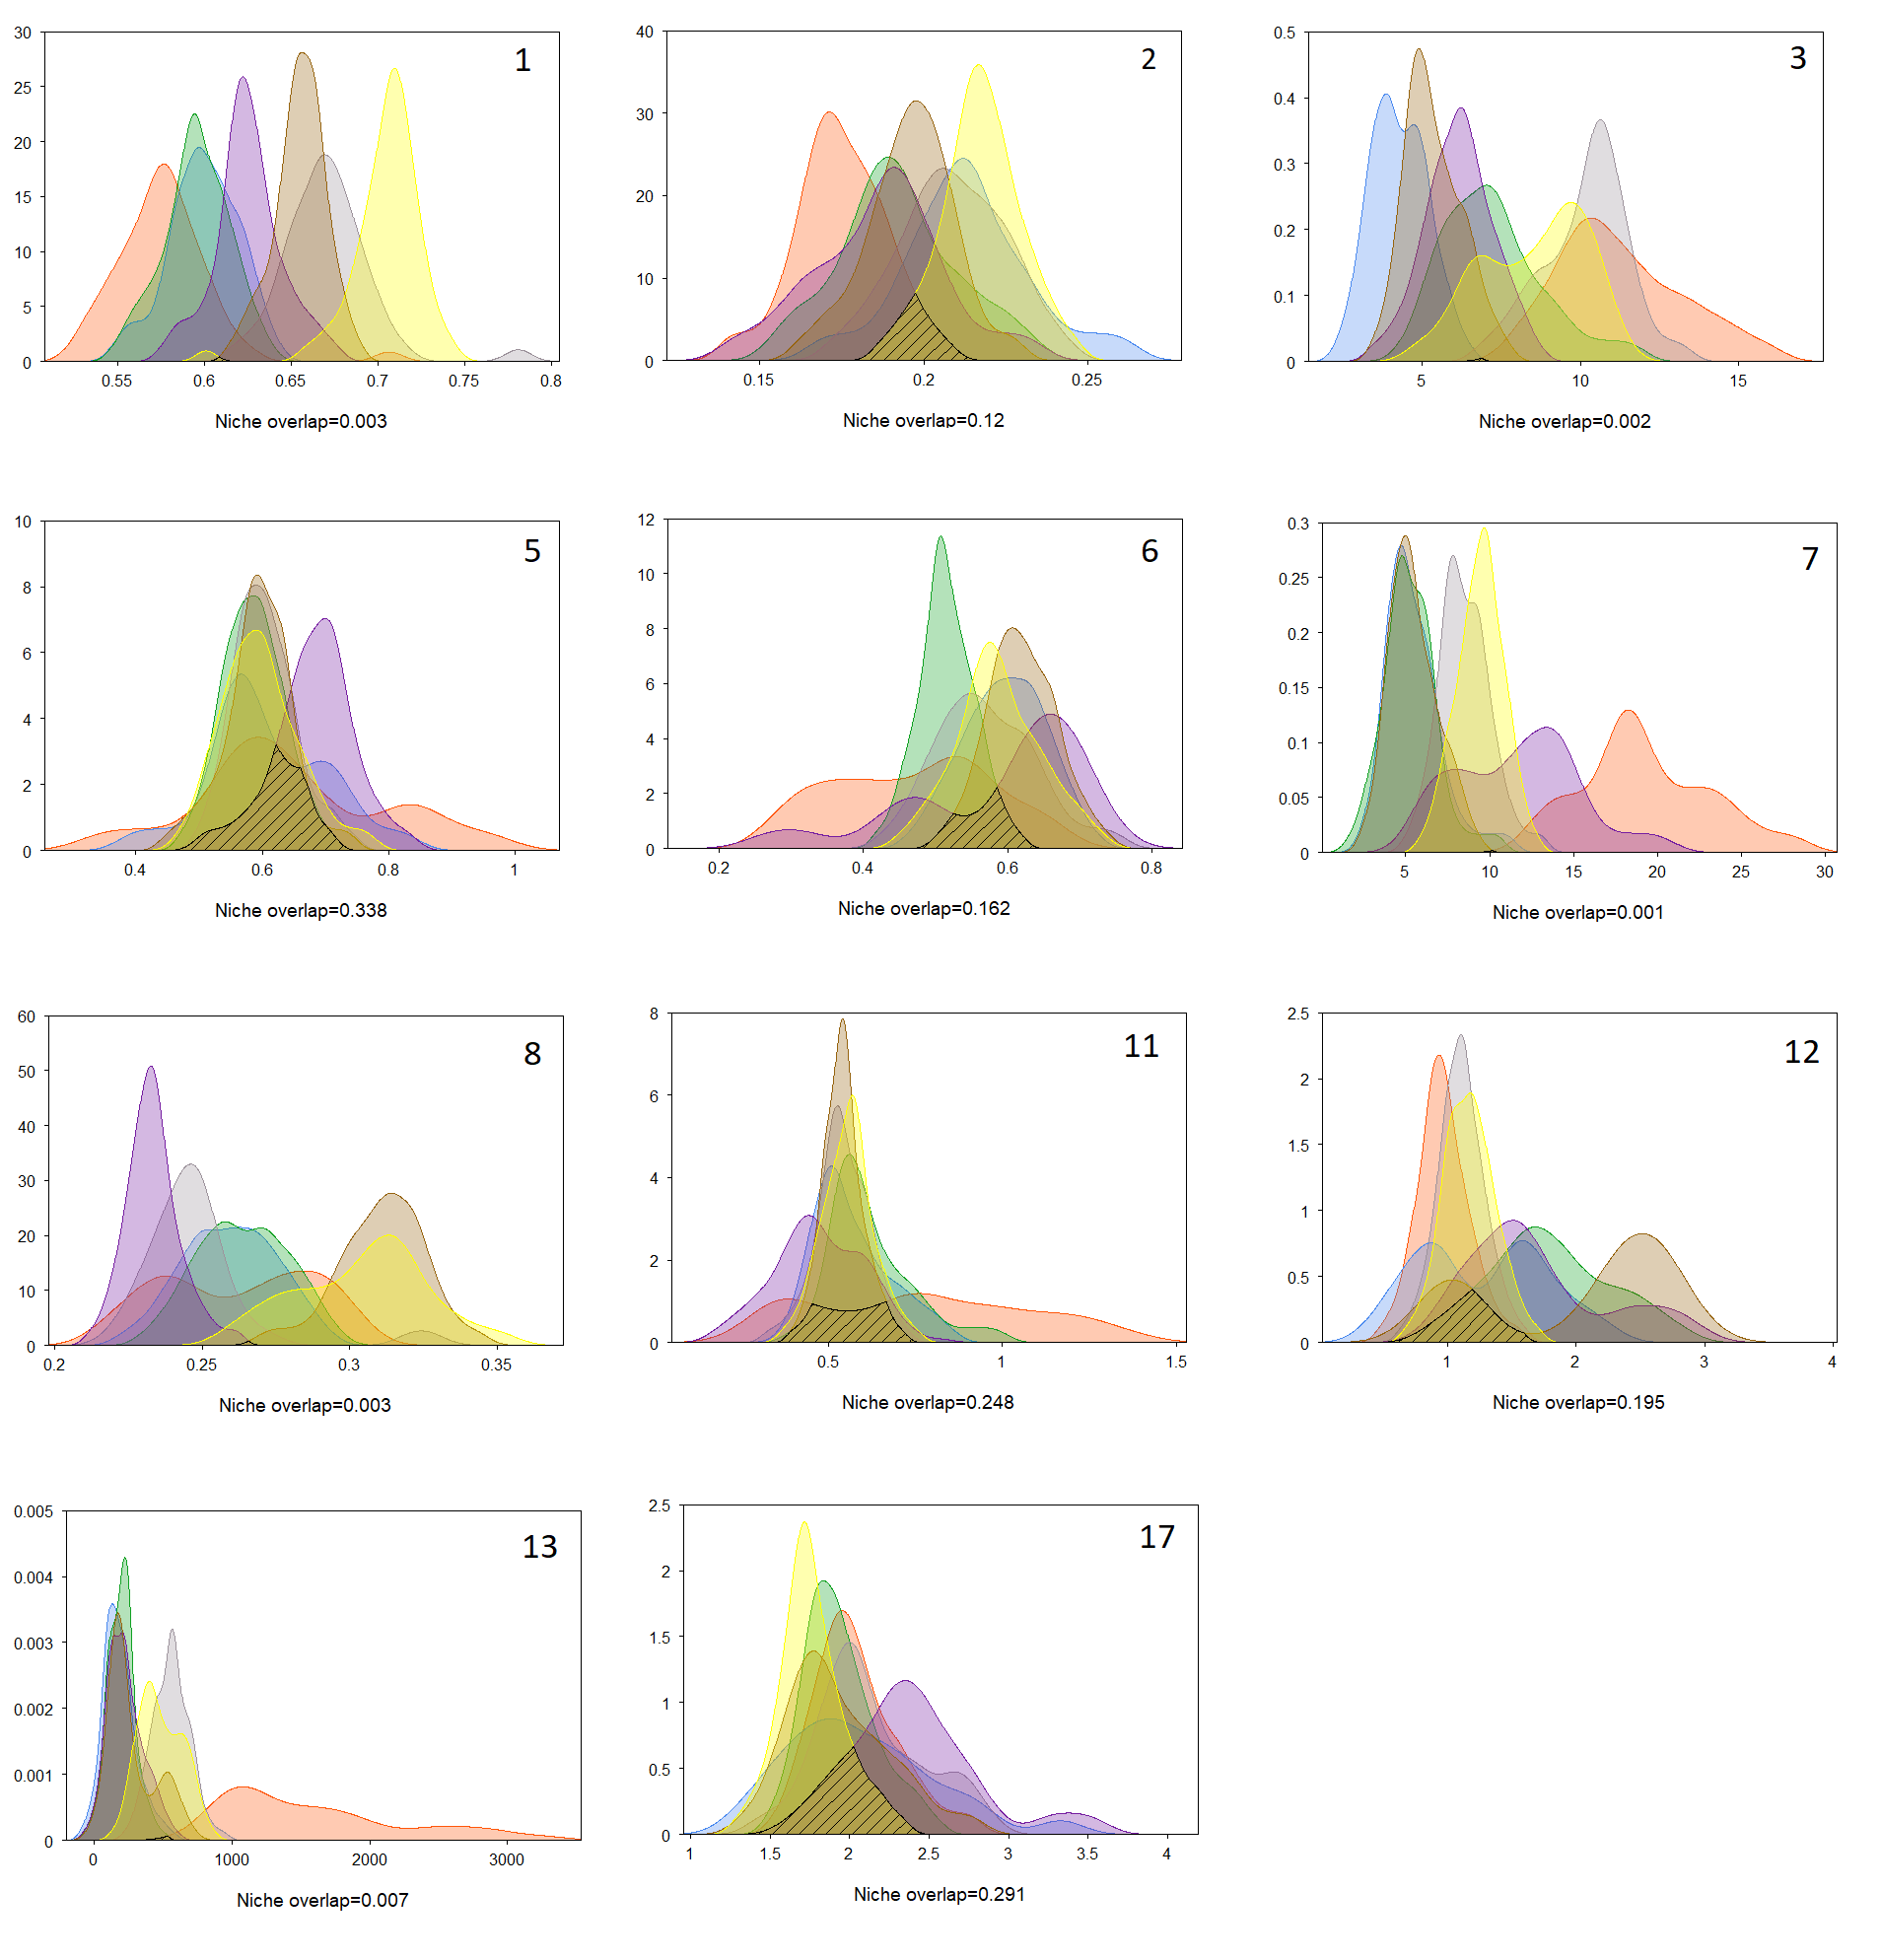
\includegraphics[width=\textwidth]{Density_plot.png}
	\end{center}
	\caption{Kernel density overlap for 11 functional traits and overlaping species. Colors correspond to following species: orange - \textit{L. crocodilus}; brown - \textit{C. maderensis}; yellow - \textit{N. operosus}; purple - \textit{X. copei}; green - \textit{N. kroyeri}; blue - \textit{M. punctatum}.}
	\label{fig:dpo}
\end{figure}